\chapter{Pertemuan 2}


%Belum Dikerjakan 
\section{Issues \#21}
Pada \textit{issues \#21} (\textit{Error: Cannot Resolve Symbol}) \textit{Cannot Resolve symbol} 

\section{Issues \#22}
Pada \textit{issues \#22} (Test Notifikasi) issues ini berisi test dari notifikasi yang sudah berjalan. Notifikasi ini menggunakan method Notiftest yang diletakan pada mainActivity.java.
\begin{verbatim}
public void Notiftest(View view) {
NotificationCompat.Builder builder = new NotificationCompat.Builder(this)
        .setSmallIcon(R.mipmap.ic_launcher)
           .setContentTitle("Issues Notif")
        .setAutoCancel(true)
        .setContentText("Berhasil Pak");
    NotificationManager notificationManager = (NotificationManager)getSystemService(Context.NOTIFICATION_SERVICE);
    notificationManager.notify(NOTIFICATION_ID,builder.build());
}
\end{verbatim}

\section{Issues \#23}
Pada \textit{issues \#23} (Membuat layout pemasukan dan pengeluaran)layout dibuat dalam file xml dengan memasukan tombol-tombol dan inputan text. Dalam pembuatan layout ini menggunakan cara \textit{Drag and Drop} melalui opsi yang sudah disediakan oleh android studio dan menghasilkan tampilan seprti: 
\begin{figure}
    \centering
    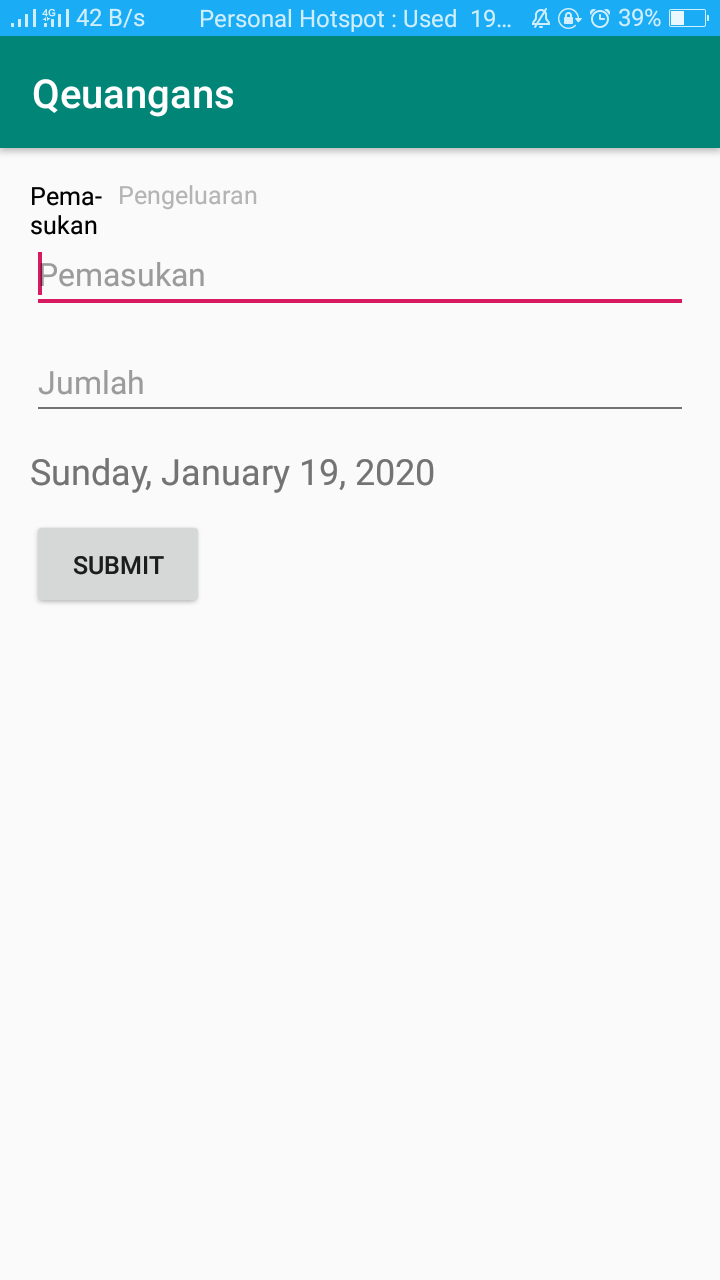
\includegraphics[scale = 0.3]{pictures/pemasukan_layout.png}
    \caption{Gambar Layout Pemasukan}
\end{figure}
\begin{figure}
    \centering
    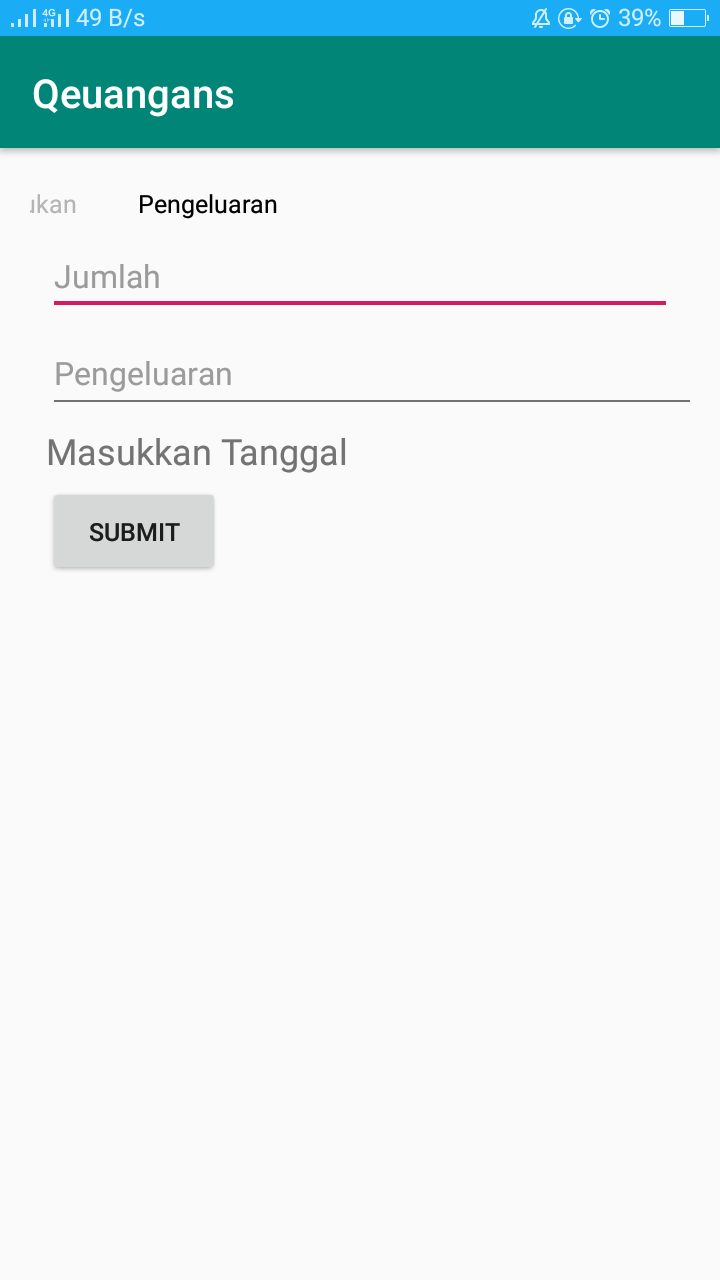
\includegraphics[scale = 0.3]{pictures/pengeluaran_layout.png}
    \caption{Gambar Layout Pengeluaran}
\end{figure}

\section{Issues \#24}
Pada \textit{issues \#24} (\textit{Datepicker Dialog} pada input pengeluaran). \textit{Datepicker} merupakan fasilitas yang disediakan android untuk memilih tanggal. Untuk menggunakan \textit{datepicker} menggunakan baris kode seperti berikut:
\begin{verbatim}
final int year = calendar.get(Calendar.YEAR);
final int month = calendar.get(Calendar.MONTH);
final int day = calendar.get(Calendar.DAY_OF_MONTH);

tglpengeluaran.setOnClickListener(new View.OnClickListener() {
    @Override
    public void onClick(View view) {
        DatePickerDialog datepickerdialog = new DatePickerDialog(InputData2.this,
                android.R.style.Theme_Holo_Light_Dialog_MinWidth,setListener,year,month,day);
        datepickerdialog.getWindow().setBackgroundDrawable(new ColorDrawable(Color.TRANSPARENT));
        datepickerdialog.show();
    }
});
setListener = new DatePickerDialog.OnDateSetListener() {
    @Override
    public void onDateSet(DatePicker datePicker, int year, int month, int dayOfMont) {
        month = month+1;
        String date = day+"/"+month+"/"+year;
        tglpengeluaran.setText(date);
    }
};
\end{verbatim}

\section{Issues \#25}
Pada \textit{issues \#25} (Mengubah Pungsi Pada Pemasukan). Pengubahan fungsi ini dilakukan pada InputData.java karena layout pemasukan dan pengeluaran yang dibagi menjadi dua.

\section{Issues \#26} 
Pada \textit{issues \#26} (\textit{Error: Cannot Resolve Symbol 'jenispengeluaran'})
\begin{verbatim}
private void AddData() {
    inputmasuk.setOnClickListener(
            new View.OnClickListener() {
                @Override
                public void onClick(View view) {
                        boolean isInseted = myDB.insertData(jenispemasukan.getText().toString(),
                                jmlpemasukan.getText().toString(), **jenispengeluaran** .getText().toString(),
                                jmlpengeluaran .getText().toString(), tglpemasukan.getText().toString());
                        if (isInseted = true)
                            Toast.makeText(InputData.this, "INPUT BERHASIL", Toast.LENGTH_LONG).show();
                        else
                            Toast.makeText(InputData.this, "INPUT GAGAL", Toast.LENGTH_LONG).show();

                }
            }
\end{verbatim}
Error ini terjadi karena method \textit{insertData} pada \textit{DatabaseHelper.java} tidak ada perintah untuk melakukan inputan jenispengeluaran sehingga pada method AddData() diatas terjadi \textit{error cannot resolve symbol}. Solusinya adalah dengan menghapus jenispengeluaran pada method AddData.
\begin{verbatim}
private void AddData() {
    inputmasuk.setOnClickListener(
            new View.OnClickListener() {
                @Override
                public void onClick(View view) {
                        boolean isInseted = myDB.insertData(jenispemasukan.getText().toString(),
                                jmlpemasukan.getText().toString(), tglpemasukan.getText().toString());
                        if (isInseted = true)
                            Toast.makeText(InputData.this, "INPUT BERHASIL", Toast.LENGTH_LONG).show();
                        else
                            Toast.makeText(InputData.this, "INPUT GAGAL", Toast.LENGTH_LONG).show();

                }
            }
\end{verbatim}

\section{Issues \#27}
Pada \textit{issues \#27} (Menambahkan \textit{Current Date} pada Input Pemasukan (InputData.java)). Current Date disini merupakan tanggal pada hari ini, cara menambahkannya dengan menambahkan baris perintah
\begin{verbatim}
Calendar calendar = Calendar.getInstance();
String currentDate = DateFormat.getDateInstance(DateFormat.FULL).format(calendar.getTime());
\end{verbatim}
pada InputData.java

\section{Issues \#28}
Pada \textit{issues \#28} (Menambahkan \textit{Casting} pada InputData2.java) casting ini dilakukan untuk mensingkronisasi view pada file activity\_InputData2.XML dengan InputData2.java.
\begin{verbatim}
jenispengeluaran = findViewById(R.id.jenispengeluaran);
\end{verbatim}
jenis pengeluaran disini merupakan \textit{variable} yang dapat dipanggil. Dalam \textit{variable} tersebut terdapat \textit{findViewById} yang digunakan untuk mencari view pada activity\_InputData2.XML dan \textit{R.id.jenispengeluaran} merupakan id dari view yang akan di sinkronisasi pada activity\_InputData2.XML


\section{Issues \#29}
Pada \textit{issues \#29}

\section{Issues \#30}
Pada \textit{issues \#30}